\section{The current state of \knox{}} \label{currentState}
\subsection{Server Distribution and Their Specifications}
The \knox{} server system consists of six servers, each having the Ubuntu 18.04 LTS operating system installed. The servers each have 4 GiB of RAM, 2 vCPUs, and about 100 GB of hard drive space. 

Four of these nodes have no ports open to public, and serve as containers for running the various applications of the \knox{} pipeline.
These servers will be referred to as \textit{node servers} or \textit{server nodes}.
The remaining two servers have port 80 and 443 open to public. These nodes will be referred to as \textit{master nodes}.
Currently, one of the master nodes run Grafana\cite{GRAFANA}, Prometheus\cite{Prometheus}, Apache\cite{ApacheJena}, and Docker\cite{Docker_IBM}.
The other master node only have a single running program, NMap\cite{NMap}.
The Docker instance runs containers based on images of Portainer, Wiki.JS, as well as a PostgreSQL database.
Many of the node servers runs applications written in Java and Python, as well as databases for the applications. 
No firewalls are set in place between the servers.

Having established an overview of the programs and running on the servers, we will now take a closer look at the databases of the third pipeline layer.


\input{sections/Chapter 3 Sprint 1/PostgreSQL.tex}
\subsection{The current \knox{} databases}
\subsubsection*{Postgres database}
To summarize, the previous group set up a PostgreSQL database on \texttt{node02}.

Figure \ref{olddatabase} shows an ER diagram of the database as we received it from the previous group.

\begin{figure}[h]
    \centering
    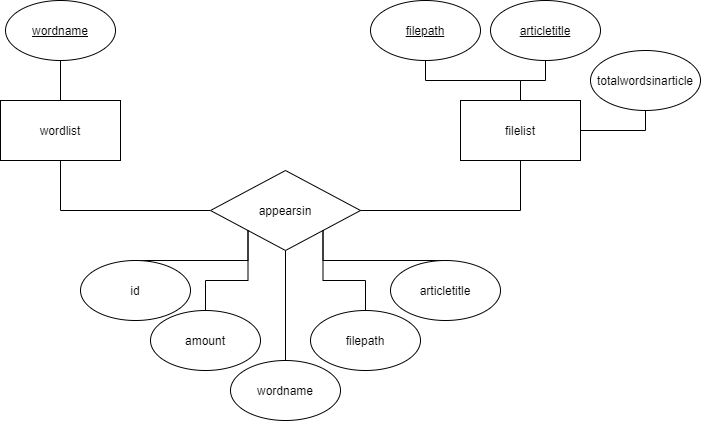
\includegraphics[width=\linewidth]{Images/old_db_er_diagram.png}
    \caption{ER diagram of the relational database from last year.}
    \label{olddatabase}
\end{figure}

\subsubsection*{Fuseki database}
The previous group set Apache Jena Fuseki on \texttt{node01}. They chose to use HDT format, claiming that it is faster for querying than TDP\cite{knox2020}.

The setup is used to store the knowledge graph used in \knox{}.

\subsection{Database endpoints and implemented applications}

As previously mentioned, \knox{} was initially started in 2020.
The previous group chose to develop API endpoints using Java.
They set up a simple database system using the Apache Jena framework in combination with the Fuseki package.

The system has two functionalities. 
First, it can store knowledge graphs in HDT and convert triples to HDT.
Second, it contains a prototype for counting the number of words in an article.
There is no API for reading this data, only for writing. 
In addition, at least one of other layers are directly connected to the database.

Overall, not much code was written, and its quality is unknown due to a lack of testing and documentation.
The Java language convention was also not followed \cite{java_convention}, making it difficult to comprehend.
It appears as though no structure was established, making it difficult to navigate the code. 
Furthermore, the database is set up such that it must be restarted every time new data is written to it - otherwise, the data cannot be fetched by the other layers.

Based on this, we have discussed what work to do and in what order.
After having read and understood the current code, we will have to start by cleaning up the inconsistencies and structure.
We will then have to document what the code does and write tests for it.
We must also address the unfortunate database implementation such that constantly restarting is no longer required.
Finally, we need to decouple the other layers such that they are no longer directly connected to the database.

To solve these issues, it was decided that the best approach was to discard all current implementations. 
This decision was based on several factors such as unfamiliarity with the environment and the previously mentioned poor structure. 
Discarding the current implementation also allows us to build the layer using C\#, a programming language that we are more familiar with which is also taught in the future semesters. 
This will make it easier for the following groups to continue and not have to learn a new language.

While doing so, we will follow a proper structure and write tests and documentation along the way. 
Moreover, it would make the system more accessible to future students as C\# is taught on the 3rd semester.